% All the following setup code was written by Brian Snider, Computer Science and Information Systems professor at George Fox University.

\documentclass[10pt]{exam}

\usepackage[T1]{fontenc}
\usepackage{amsmath}
\usepackage{listings}
\usepackage{tikz}
\usepackage[simplified]{pgf-umlcd}
%\usepackage{ulem}
\usepackage{url}


% listings:  format code samples
\lstset{
  language=Java,
  basicstyle=\small\ttfamily,
  commentstyle=\ttfamily,
  columns=flexible,
  breaklines=true,
  breakatwhitespace=true,
  keepspaces=true,
}

% pgf-umlcd:  use guillemets for interfaces & abstract classes
\renewenvironment{interface}[3][]{\begin{classAndInterfaceCommon}{#1}{#2}{#3}}{%
  \calcuateNumberOfParts{}
  \node[this umlcd style, anchor=north] (\umlcdClassName) at (\umlcdClassPos) {%
    \footnotesize\guillemotleft\,interface\,\guillemotright\normalsize \\ \textbf{\umlcdClassName}
    \insertAttributesAndOperations{}
  };
  \end{classAndInterfaceCommon}
}
\renewenvironment{abstractclass}[3][]{\begin{classAndInterfaceCommon}{#1}{#2}{#3}}{%
  \calcuateNumberOfParts{}
  \node[this umlcd style, anchor=north] (\umlcdClassName) at (\umlcdClassPos) {%
    \footnotesize\guillemotleft\,abstract\,\guillemotright\normalsize \\ \textbf{\umlcdClassName}
    \insertAttributesAndOperations{}
  };
  \end{classAndInterfaceCommon}
}

% pgf-umlcd:  template parameters
\tikzset{
  template parameter/.style={
    append after command={
      node [draw, densely dashed, umlcolor, font=\ttfamily] at (\tikzlastnode.north east) {\footnotesize#1\normalsize}
    }
  }
}

% pgf-umlcd:  inner class associations
\usetikzlibrary{arrows.meta}
\pgfdeclarearrow{
  name=Contains,
  parameters={\the\pgfarrowlength},
  setup code={
   \pgfarrowssettipend{0pt}
   \pgfarrowssetlineend{-\pgfarrowlength}
   \pgfarrowlinewidth=\pgflinewidth
   \pgfarrowssavethe\pgfarrowlength
  },
  drawing code={
   \pgfpathcircle{\pgfpoint{-0.5\pgfarrowlength}{0pt}}{0.5\pgfarrowlength}
   \pgfpathmoveto{\pgfpoint{0.0\pgfarrowlength}{0.0\pgfarrowlength}}
   \pgfpathlineto{\pgfpoint{-1.0\pgfarrowlength}{0.0\pgfarrowlength}}
   \pgfpathmoveto{\pgfpoint{-0.5\pgfarrowlength}{0.5\pgfarrowlength}}
   \pgfpathlineto{\pgfpoint{-0.5\pgfarrowlength}{-0.5\pgfarrowlength}}
   \pgfusepathqstroke
  },
  defaults={length=7pt}
}
\tikzstyle{umlcd style associationinner}=[<-,>=Contains, umlcolor, >=angle 90]
\newcommand{\associationinner}[6]{
  \draw [<-,>=Contains] (#1) -- (#4)
  node[near start, above]{#2}
  node[near start, below]{#3}
  node[near end, above]{#5}
  node[near end, below]{#6};
}


% pgf-umlcd:  make readable for b&w printout
\renewcommand{\umltextcolor}{black}
\renewcommand{\umldrawcolor}{black}
\renewcommand{\umlfillcolor}{white}
\tikzset{every node/.append style={font=\ttfamily}}

% ulem:  set underline depth
%\renewcommand{\ULdepth}{3pt}

\begin{document}

\section*{Graph Implementation}
\subsection*{Class Diagram}

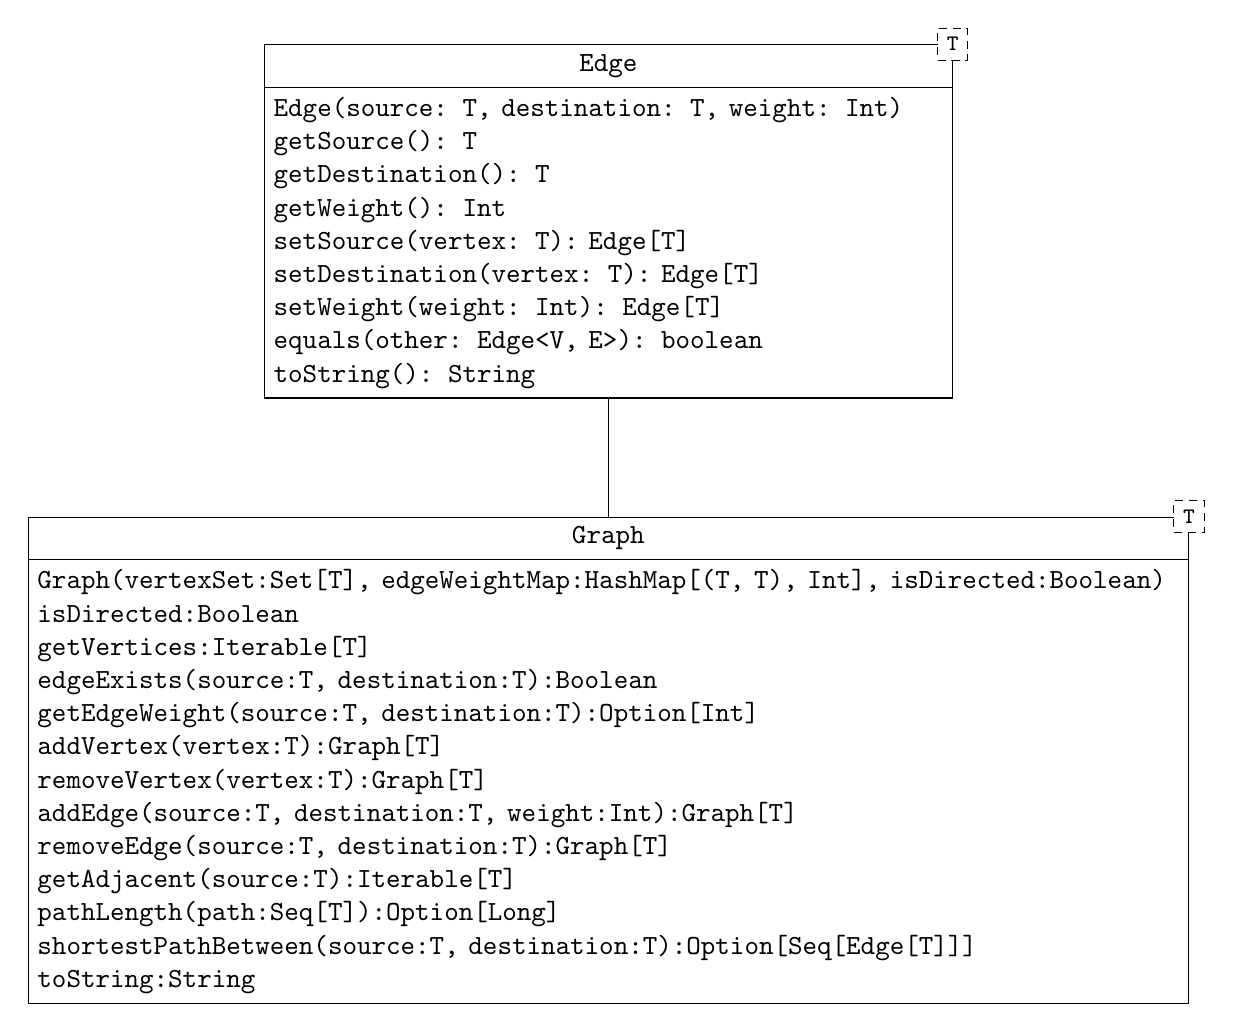
\begin{tikzpicture}
  \begin{class}[template parameter={T}, text width=8.5cm]{Edge}{0,11}
    \operation{Edge(source: T, destination: T, weight: Int)}
    \operation{getSource(): T}
    \operation{getDestination(): T}
    \operation{getWeight(): Int}
    \operation{setSource(vertex: T): Edge[T]}
    \operation{setDestination(vertex: T): Edge[T]}
    \operation{setWeight(weight: Int): Edge[T]}
    \operation{equals(other: Edge<V, E>): boolean}
    \operation{toString(): String}
  \end{class}

  \begin{class}[template parameter={T}, text width=14.5cm]{Graph}{0,5}
    \operation{Graph(vertexSet:Set[T], edgeWeightMap:HashMap[(T, T), Int], isDirected:Boolean)}
    \operation{isDirected:Boolean}
    \operation{getVertices:Iterable[T]}
    \operation{edgeExists(source:T, destination:T):Boolean}
    \operation{getEdgeWeight(source:T, destination:T):Option[Int]}
    \operation{addVertex(vertex:T):Graph[T]}
    \operation{removeVertex(vertex:T):Graph[T]}
    \operation{addEdge(source:T, destination:T, weight:Int):Graph[T]}
    \operation{removeEdge(source:T, destination:T):Graph[T]}
    \operation{getAdjacent(source:T):Iterable[T]}
    \operation{pathLength(path:Seq[T]):Option[Long]}
    \operation{shortestPathBetween(source:T, destination:T):Option[Seq[Edge[T]]]}
    \operation{toString:String}
  \end{class}

  \association{Graph}{}{}{Edge}{}{}
\end{tikzpicture}
\begin{figure}[ht]
  \centering
  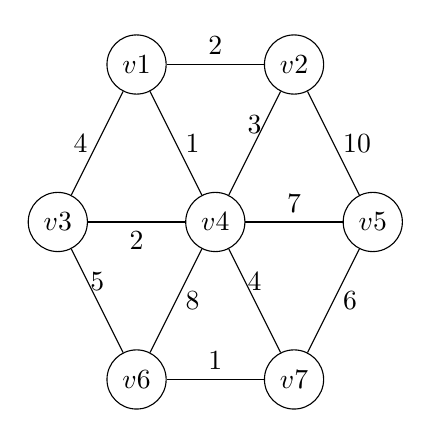
\begin{tikzpicture}
    \node[draw, shape = circle] (v1) at (1,4) {$v1$};
    \node[draw, shape = circle] (v2) at (3,4) {$v2$};
    \node[draw, shape = circle] (v3) at (0,2) {$v3$};
    \node[draw, shape = circle] (v4) at (2,2) {$v4$};
    \node[draw, shape = circle] (v5) at (4,2) {$v5$};
    \node[draw, shape = circle] (v6) at (1,0) {$v6$};
    \node[draw, shape = circle] (v7) at (3,0) {$v7$};

    \draw
      (v1) edge[above] node{$2$} (v2)
      (v1) edge[right] node{$1$} (v4)
      (v1) edge[left] node{$4$} (v3)
      (v4) edge[above] node{$3$} (v2)
      (v4) edge[above] node{$7$} (v5)
      (v4) edge[above] node{$4$} (v7)
      (v4) edge[right] node{$8$} (v6)
      (v4) edge[below] node{$2$} (v3)
      (v2) edge[right] node{$10$} (v5)
      (v5) edge[right] node{$6$} (v7)
      (v7) edge[above] node{$1$} (v6)
      (v6) edge[above] node{$5$} (v3);

  \end{tikzpicture}
  \caption{Default Graph Orr uses in class}
\end{figure}
\end{document}
